\documentclass[tikz,border=10pt]{standalone}
\usetikzlibrary{decorations.markings,quotes}
\begin{document}
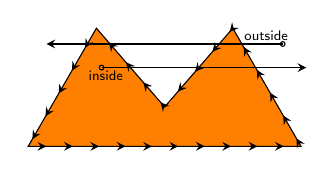
\begin{tikzpicture}[
    draw=black, fill=orange,
    decoration={markings, 
    mark = between positions 0.03 and 1 step 0.035 
        with {\arrow{stealth}}},
    every edge quotes/.style = {font=\sffamily\tiny,sloped,above,inner sep=1pt}
     ]
  \filldraw[postaction={decorate}] (150:1) -- (210:2) -- (330:2) -- (30:1) -- (0,-0.5) -- cycle;
  \draw (-0.8,0) circle[fill=black, radius=0.03]
    edge[-stealth,"inside" {pos=0.02,below}] (1.8,0);
  \draw (1.5,0.3) circle[fill=black, radius=0.03]
    edge[-stealth,"outside" pos=0.07] (-1.5,0.3);
\end{tikzpicture}
\end{document}
